\section[Glossario]{Glossario}
\sectionframe{images/covers/cover_glossary.jpg}{Glossario}


% Ottavio Calzone: Pagina 36-72 tipologie di apprendimento
\subsection[Machine learning, Statistical learning, \& Co.]{Machine learning, Statistical learning, \& Co.}


% TODO rivedere questa slide
\begin{frame}
	%\frametitle{Definizione}

	\begin{block}{Machine learning, Statistical learning, \& Co.}
		L'ambito di ricerca che affronta questa tipologia di problemi ha nomi diversi: Machine Learning (ML), Statistical Learning (SL), Data mining, Data science, Big data, ...\\
		In gran parte questi campi sono sovrapposti.\\
		Tuttavia esistono alcune differenze:
		\begin{itemize}
			\item alcune di queste discipline sono nate in dipartimenti di informatica, altre in quelli di statistica
			\item alcune applicazioni tendono a considerare campioni con dimensioni diverse, e sono meno interessate all'interpretabilità del risultato finale
			\item alcune si concentrano maggiormente su ciò che misuriamo, altre seguono semplicemente la logica che ciò che funziona anche vero
			\item Soprattutto: esistono differenze terminologiche (vedi slide seguente)
			\item ma queste discipline interagiscono e collaborano fra loro (in maniera competitiva...)
		\end{itemize}
	\end{block}

\end{frame}


\subsection[Il glossario di Tibshirani]{Il glossario di Tibshirani}
\begin{frame}

	\frametitle{Il glossario di Tibshirani}

	%\begin{block}{}
		Nel suo corso di statistica, \textbf{Rob Tibshirani}, uno statistico che si è applicato in parte anche nel ML, fornisce un \textbf{glossario} che mappa\\
		i termini del machine learning nei termini statistici:
		\begin{figure}[!htbp]
			\centering
			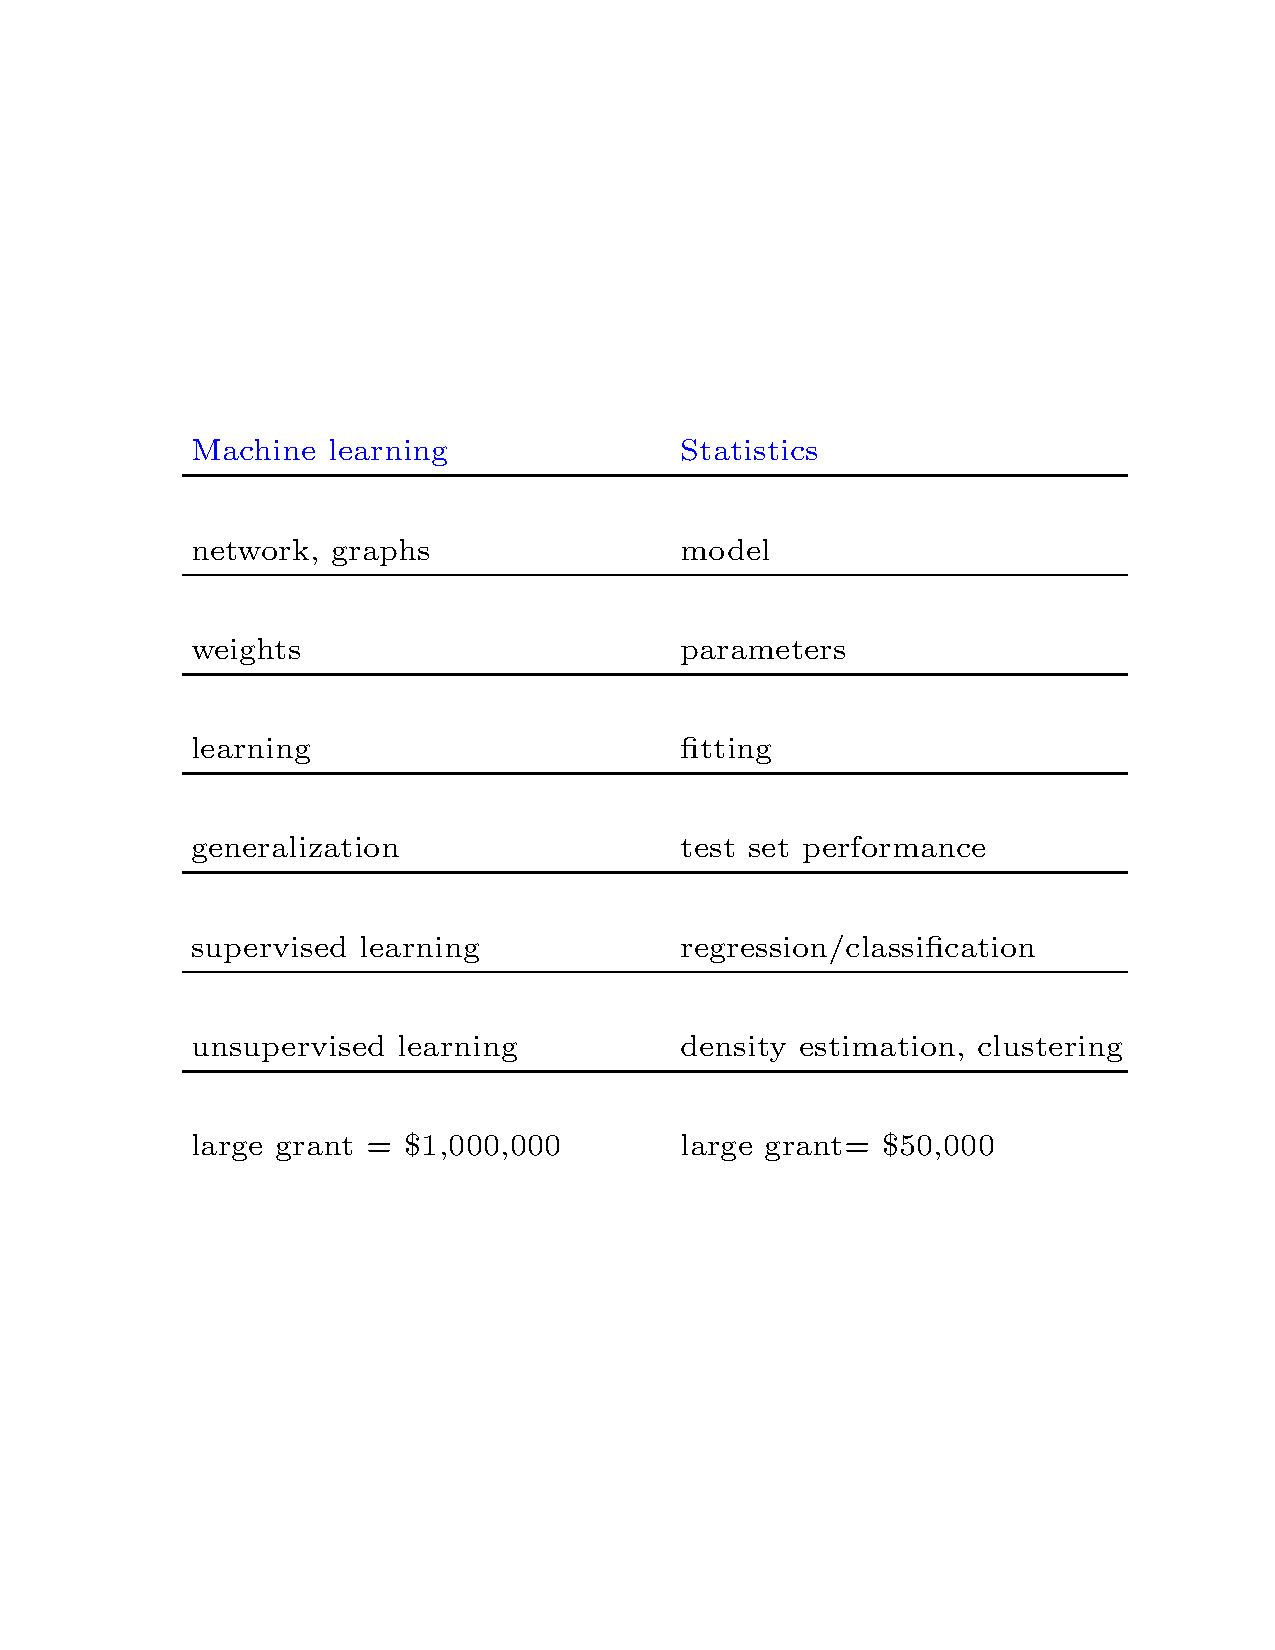
\includegraphics[width=6.5cm]{images/glossary/tibshirani_glossary.pdf}
			%\caption{Stripe Radar for Fraud Detection}
		\end{figure}
	%\end{block}


\end{frame}


\begin{frame}

	% Il \ml è Computational Applied Statistics
	\begin{block}{Come funziona il Machine Learning?}
		Dal momento che il ML considera il \textbf{mondo} stesso \textbf{rappresentabile} come \textbf{formule matematiche e statistiche}, i suoi algoritmi tentano di conoscere meglio tali formule inferendole da un numero di osservazioni limitato.
		\newlinedouble
		Come per un essere umano, non è necessario vedere prima tutti gli alberi che esistono nel mondo per riconoscerne uno (dal momento che gli esseri umani sono in grado di imparare quali sono le loro caratteristiche distintive); allo stesso modo, basandosi unicamente su un numero finito di esempi, gli algoritmi di machine learning possono usare la potenza di calcolo dei computer e l'abbondanza di dati, riguardanti praticamente qualsiasi argomento, per imparare a risolvere un enorme numero di problemi importanti e la cui soluzione riveste una notevole utilità per tutti noi.
		 \vskip5mm
		\hspace*\fill{\small--- \textit{Machine Learning for Dummies - Massaron e Mueller} }
	\end{block}


\end{frame}


\subsection[Features]{Features}
\begin{frame}

	\frametitle{Glossario}
	\framesubtitle{introduciamo alcuni termini ricorrenti nel \ml}

	\begin{block}{Features}
		Una \textbf{feature} (in italiano  \textbf{caratteristica}) è una variabile di input,\\
		ad esempio la variabile $\textbf{x}$ nella regressione lineare semplice.\\
		\vspace{1.8mm}
		Un progetto semplice potrebbe utilizzare anche una singola \textbf{feature}, mentre un progetto più complesso potrebbe utilizzare anche milioni di \textbf{features}, specificate come:\\
  			\makebox[\textwidth]{$\textbf{x}_{\textbf{1}}, \textbf{x}_{\textbf{2}},..., \textbf{x}_{\textbf{N}}$}\\
		\vspace{1.8mm}
		\pause
		Nell'esempio del rilevatore di spam, le \textbf{features} potrebbero includere:
		\begin{itemize}
			\pause
			\item il numero di parole nel testo dell'email
			\pause
			\item l'indirizzo del mittente
			\pause
			\item l'ora del giorno in cui è stata inviata l'email
			\pause
			\item l'email contiene la frase ``one weird trick''.
		\end{itemize}

	\end{block}

\end{frame}


\begin{frame}

	\frametitle{Glossario}
	\framesubtitle{introduciamo alcuni termini ricorrenti nel \ml}

	\begin{block}{}
		Le \textbf{features} possono essere:
		\begin{itemize}
			\item \textbf{quantitative}: valori numerici, rappresentanti misure
			\item \textbf{qualitative}: dette anche \textbf{categoriche/discrete/fattori}:\\
				stringhe di testo rappresentanti delle qualità
		\end{itemize}
		\pause
		
		\begin{columns}
			\column{0.55\linewidth}
			
			\begin{figure}[!htbp]
				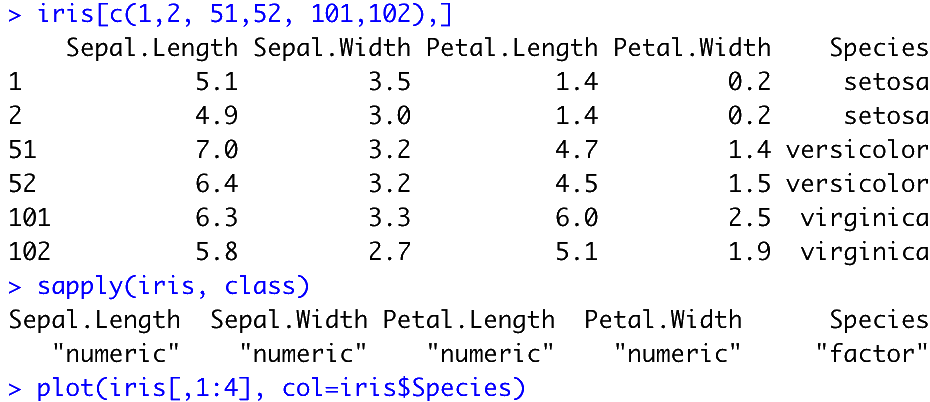
\includegraphics[width=1.0\linewidth]{images/glossary/iris_1.png}
				%\caption{}
			\end{figure}
			
%			\column{0.45\linewidth}
%			\begin{figure}[!htbp]
%				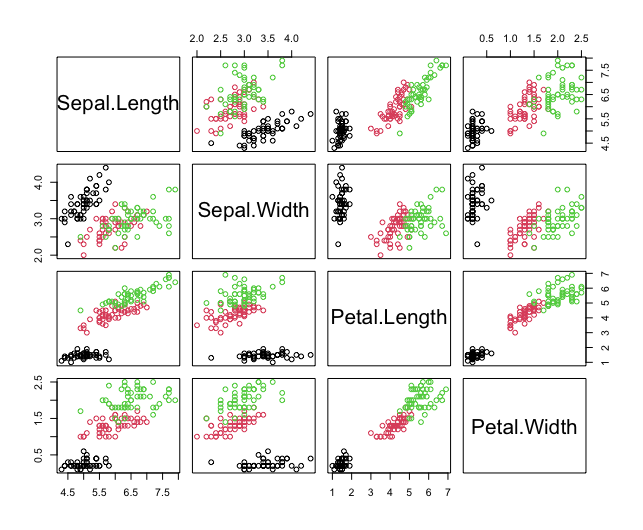
\includegraphics[width=1.0\linewidth]{images/glossary/iris_2.png}
%				%\caption{}
%			\end{figure}
		\end{columns}
		
	\end{block}

\end{frame}





\begin{frame}

	\frametitle{Glossario}
	\framesubtitle{introduciamo alcuni termini ricorrenti nel \ml}
	
		\href{https://en.wikipedia.org/wiki/Iris_flower_data_set}{\underline{\textbf{Iris Flower Data Set}}}: esempio di estrazione di features quantitative		
		
		\begin{figure}[!htbp]
			\centering
				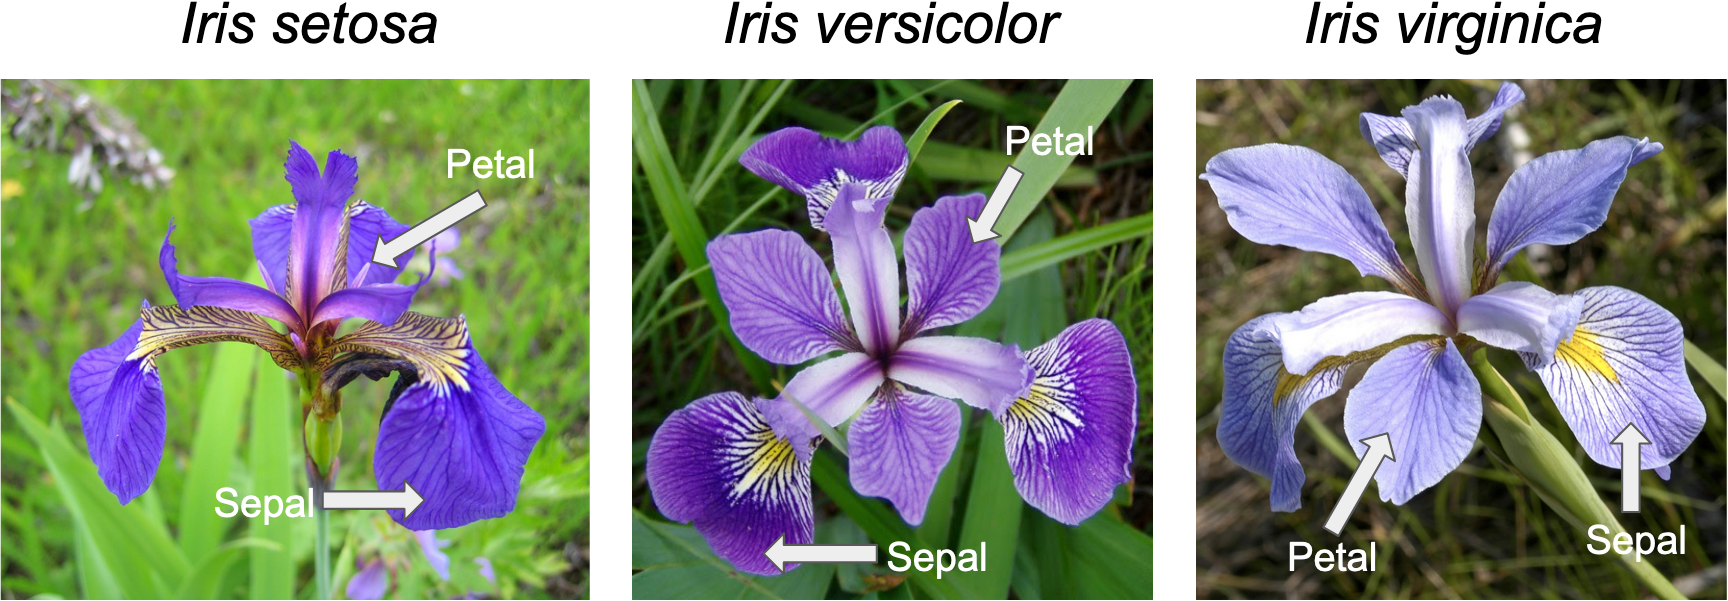
\includegraphics[width=0.75\linewidth]{images/glossary/iris_petal_sepal.png}
				%\caption{Stripe Radar for Fraud Detection}
			\end{figure}
		\pause
		
		\begin{columns}
			\column{0.4\linewidth}
			
			\begin{figure}[!htbp]
				\hspace{15mm}
				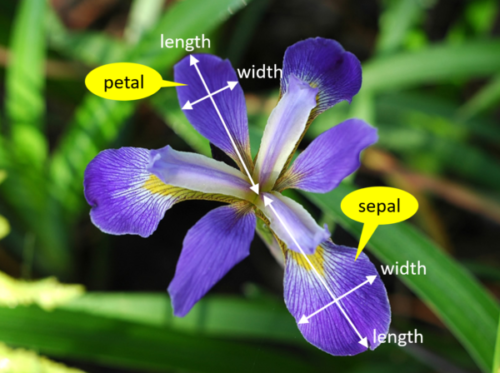
\includegraphics[width=0.65\linewidth]{images/glossary/iris_petal_sepal_features.png}
				
				%\caption{}
			\end{figure}
			
			\pause
			\column{0.01\linewidth}
			\begin{large}
				\vspace{5mm}
				$$\pmb{\Rightarrow}$$
			\end{large}
			
			\column{0.59\linewidth}
			\begin{figure}[!htbp]
				\centering
				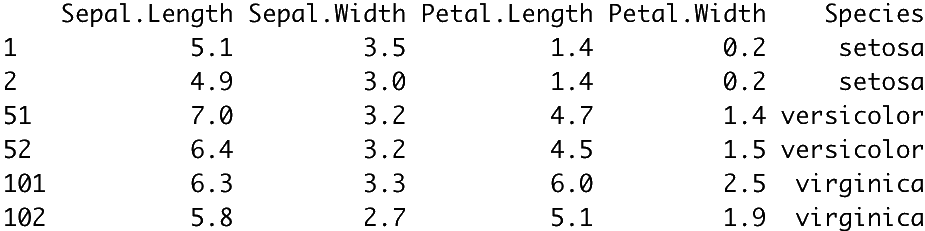
\includegraphics[width=0.85\linewidth]{images/glossary/iris_3.png}
				%\caption{}
			\end{figure}	
		\end{columns}


\end{frame}





\subsection[Labels]{Labels}
\begin{frame}

	\frametitle{Glossario}
	\framesubtitle{introduciamo alcuni termini ricorrenti nel \ml}

	\begin{block}{Labels}
		Una \textbf{label} o \textbf{classe} è ciò vogliamo predire con il nostro modello di ML:\\
		ad esempio la variabile $y$ nella regressione lineare semplice.
		\newlinedouble
		\pause
		Una \textbf{label} potrebbe essere:
		\begin{itemize}
			\pause
			\item spam oppure non spam
			\pause
			\item la tipologia di iris: setosa, versicolor o virginica
			\pause
			\item il tipo di animale mostrato in un'immagine
			\pause
			\item il prezzo futuro del grano
			\pause
			\item la temperatura esterna
			\pause
			\item ...
		\end{itemize}
	\end{block}

\end{frame}


\begin{frame}

	\frametitle{Glossario}
	\framesubtitle{introduciamo alcuni termini ricorrenti nel \ml}

	\begin{figure}[!htbp]
		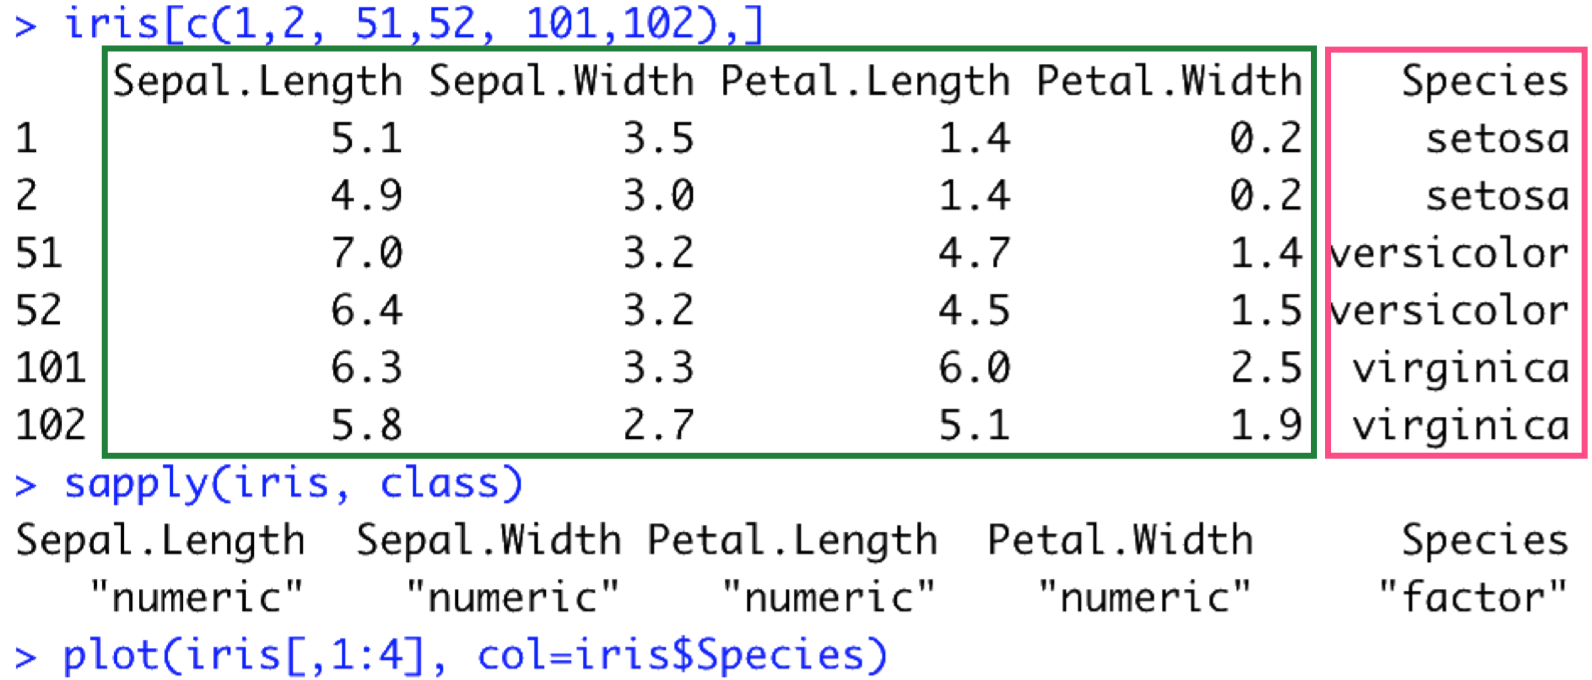
\includegraphics[width=1.0\linewidth]{images/glossary/iris_4.png}
		%\caption{}
	\end{figure}


\end{frame}



\subsection[Examples]{Examples}
\begin{frame}

	\frametitle{Glossario}
	\framesubtitle{introduciamo alcuni termini ricorrenti nel \ml}

	\begin{block}{Examples}
		Un \textbf{esempio} (example) è una particolare istanza di dati, \textbf{x}\\
		(mettiamo x in grassetto per indicare che si tratta di un vettore).
		\newlinedouble
		Dividiamo gli \textbf{esempi} in due categorie:
		\begin{itemize}
			\item esempi etichettati (labeled examples)
			\item esempi non etichettati (unlabeled examples)
		\end{itemize}

	\end{block}

\end{frame}


\subsubsection[Labeled Examples]{Labeled Examples}
\begin{frame}

	\frametitle{Glossario}
	\framesubtitle{introduciamo alcuni termini ricorrenti nel \ml}

	\begin{block}{Labeled Examples}
		Un \textbf{labeled example} (esempio etichettato)\\
		include sia la(le) caratteristica(e) che l'etichetta,\\
		ovvero:
		\newlinedouble
		\makebox[\textwidth]{\textbf{labeled examples: \{features, label\}: (x, y)}}
		\newlinedouble

		Nel nostro esempio del rilevamento dello spam, gli esempi etichettati sarebbero singole email che gli utenti hanno esplicitamente contrassegnato come ``spam'' o ``non spam''.

	\end{block}

\end{frame}


\begin{frame}

	\frametitle{Glossario}
	\framesubtitle{introduciamo alcuni termini ricorrenti nel \ml}

	\begin{block}{Labeled Examples}
		Ad esempio, la seguente tabella mostra 5 \textbf{esempi etichettati} presi da un dataset contenente informazioni sui prezzi delle case in California:
		\newlinedouble

	% Text size https://texblog.org/2012/08/29/changing-the-font-size-in-latex/
	\begin{scriptsize}
		\begin{table}
		\begin{tabular}{|c|c|c|c|}
		\hline
		\rowcolor{gray!25} \textbf{housingMedianAge} & \textbf{totalRooms} & \textbf{totalBedrooms} & \textbf{medianHouseValue} \\
		\rowcolor{gray!25} \textbf{(feature)} & \textbf{(feature)} & \textbf{(feature)} & \textbf{(label)} \\ \hline
		\textit{15} & \textit{5612} & \textit{1283} & \cellcolor{yellow!15} \textit{66900} \\ \hline
		\textit{19} & \textit{7650} & \textit{1901} & \cellcolor{yellow!15}\textit{80100} \\ \hline
		\textit{17} & \textit{720} & \textit{174} & \cellcolor{yellow!15}\textit{85700} \\ \hline
		\textit{14} & \textit{1501} & \textit{337} & \cellcolor{yellow!15}\textit{73400} \\ \hline
		\textit{20} & \textit{1454} & \textit{326} & \cellcolor{yellow!15}\textit{65500} \\ \hline
		\end{tabular}
		\end{table}
	\end{scriptsize}

	\end{block}

\end{frame}


\subsubsection[Unlabeled Examples]{Unlabeled Examples}
\begin{frame}

	\frametitle{Glossario}
	\framesubtitle{introduciamo alcuni termini ricorrenti nel \ml}

	\begin{block}{Unlabeled Examples}
		Un \textbf{unlabeled example} (esempio non etichettato)\\
		contiene la(le) caratteristica(e) ma non l'etichetta,\\
		ovvero:
		\newlinedouble
		\makebox[\textwidth]{\textbf{unlabeled examples: \{features, ?\}: (x, ?)}}

	\end{block}

\end{frame}



\begin{frame}

	\frametitle{Glossario}
	\framesubtitle{introduciamo alcuni termini ricorrenti nel \ml}

	\begin{block}{Unlabeled Examples}
		Di seguito sono riportati 3 \textbf{esempi senza etichetta} dello stesso dataset riguardante le case in California, che escludono \textbf{medianHouseValue}:

			% Text size https://texblog.org/2012/08/29/changing-the-font-size-in-latex/
		\begin{scriptsize}
			\begin{table}
			\begin{tabular}{|c|c|c|c|}
			\hline
			\rowcolor{gray!25} \textbf{housingMedianAge} & \textbf{totalRooms} & \textbf{totalBedrooms} & \textbf{medianHouseValue} \\
			\rowcolor{gray!25} \textbf{(feature)} & \textbf{(feature)} & \textbf{(feature)} & \textbf{(label)} \\ \hline
			\textit{42} & \textit{1686} & \textit{361} & \cellcolor{yellow!15}\textit{?} \\ \hline
			\textit{34} & \textit{1226} & \textit{180} & \cellcolor{yellow!15}\textit{?} \\ \hline
			\textit{33} & \textit{1077} & \textit{271} & \cellcolor{yellow!15}\textit{?} \\ \hline
			\end{tabular}
			\end{table}
		\end{scriptsize}

		Dopo aver addestrato il nostro modello con esempi etichettati, utilizziamo quel modello per prevedere l'etichetta su esempi senza etichetta.
		\newlinedouble
		Nel rilevatore di spam, esempi senza etichetta sono le nuove e-mail che gli esseri umani non hanno ancora etichettato (come ``spam'' o ``non spam'').
	\end{block}

\end{frame}


\subsection[Funzione target]{Funzione target}
% TODO Rileggere: funzione target...
\begin{frame}

	\frametitle{Glossario}
	\framesubtitle{introduciamo alcuni termini ricorrenti nel \ml}

	\begin{block}{Funzione target}

		Un bambino  astrae l’idea di come dovrebbe essere un albero confrontando le caratteristiche (feature) con le immagini di altri oggetti diversi.\\
		\vspace{2mm}
		 %, per esempio mobili che, pur essendo fatti di legno, non condividono con l’albero le altre caratteristiche.\\

		Un classificatore di machine learning funziona alla stessa maniera: le sue capacità cognitive vengono costituite sviluppando una formula matematica che comprenda tutte le feature fornite, in modo da arrivare ad avere una funzione che sia in grado di distinguere una classe dall’altra.\\
		\vspace{3mm}

		Supponiamo che esista una formula matematica, nota anche come \textbf{funzione target}, in grado di esprimere le caratteristiche di un albero.\\
		\vspace{2mm}
		Essere in grado di esprimere tale formula matematica costituisce quella che si chiama la \textbf{capacità rappresentativa} del classificatore.
	\end{block}

\end{frame}


\subsection[Ottimizzazione e spazio delle ipotesi]{Ottimizzazione e spazio delle ipotesi}
\begin{frame}

	\frametitle{Glossario}
	\framesubtitle{introduciamo alcuni termini ricorrenti nel \ml}

	\begin{block}{Ottimizzazione e spazio delle ipotesi}
		Durante l’\textbf{ottimizzazione} (il processo di calcolo dell’ottimizzatore), l’algoritmo svolge ricerche fra le possibili varianti delle combinazioni di parametri, per trovare quella migliore che consenta, nella fase di addestramento, una mappatura corretta tra le feature e le classi.\\
		\vspace{3mm}
		Questo processo calcola svariate possibili funzioni target fra quelle che l’algoritmo di apprendimento è in grado di scovare (\textbf{spazio delle ipotesi}).\\
		\vspace{3mm}
		Il classificatore risultante, unitamente a tutti i parametri impostati, prende il nome di \textbf{ipotesi}, che è un modo per dire, nel gergo del machine learning, che l’algoritmo ha impostato i parametri così da replicare la funzione target e ora è pronto a elaborare le classificazioni in modo corretto.
	\end{block}

\end{frame}


\subsection[Loss]{Loss}


\begin{frame}

	\frametitle{Glossario}
	\framesubtitle{introduciamo alcuni termini ricorrenti nel \ml}

	\begin{block}{Loss}
		Nel processo di ottimizzazione nel machine learning è la risposta da parte di una funzione interna all’algoritmo, chiamata \textbf{loss} (anche detta: \textit{funzione di costo}, \textit{funzione di perdita}, \textit{funzione obiettivo}, \textit{funzione di score} o \textit{funzione d’errore}), a giocare un ruolo di primo piano.\\
		\vspace{3mm}
		La \textbf{loss} è una funzione di valutazione che misura la capacità dell’algoritmo di machine learning di mappare la funzione target che sta cercando di individuare.\\
		\vspace{3mm}
		La \textbf{loss} opera mettendo a confronto le previsioni di un algoritmo con l’effettivo esito registrato nel mondo reale. Confrontare una previsione con il valore reale utilizzando una funzione di costo consente di stabilire il livello di errore dell’algoritmo.%\\
		%\vspace{3mm}
		%È la funzione di costo a stabilire il successo di un’applicazione di machine learning: per quanto riguarda il processo di apprendimento, tale funzione è fondamentale tanto quanto la rappresentazione (che è la capacità di approssimare determinate funzioni matematiche) e l’ottimizzazione (il modo in cui gli algoritmi di machine learning impostano al meglio i propri parametri interni)
	\end{block}

\end{frame}


\subsection[Modello]{Modello}
\begin{frame}

	\frametitle{Glossario}
	\framesubtitle{introduciamo alcuni termini ricorrenti nel \ml}

	\begin{block}{Modello}
		Un \textbf{modello} definisce la relazione tra le features e la label.\\
		\vspace{2mm}
		%Ad esempio, un modello per il rilevamento dello spam potrebbe associare fortemente determinate feature allo ``spam''.\\
		%\vspace{2mm}
		Evidenziamo le due fasi della vita di un modello:
		\begin{itemize}
			\item \textbf{Training} significa creare o addestrare il modello.\\
					Ovvero, mostri al modello degli esempi etichettati e consenti al modello di apprendere gradualmente quale sia la relazione tra le caratteristiche e l'etichetta.
			\item \textbf{Inferenza} significa applicare il modello addestrato a esempi senza etichetta.\\
				Ovvero, si utilizza il modello addestrato per eseguire previsioni utili (\textbf{y'}). Ad esempio, applicando l'inferenza, è possibile prevedere medianHouseValue per nuovi esempi senza etichetta.
		\end{itemize}

	\end{block}

\end{frame}


\begin{frame}

	\frametitle{Glossario}
	\framesubtitle{introduciamo alcuni termini ricorrenti nel \ml}

	\begin{block}{Modello (il caso classico dell'apprendimento supervisionato)}
		\begin{figure}[!htbp]
			\centering
			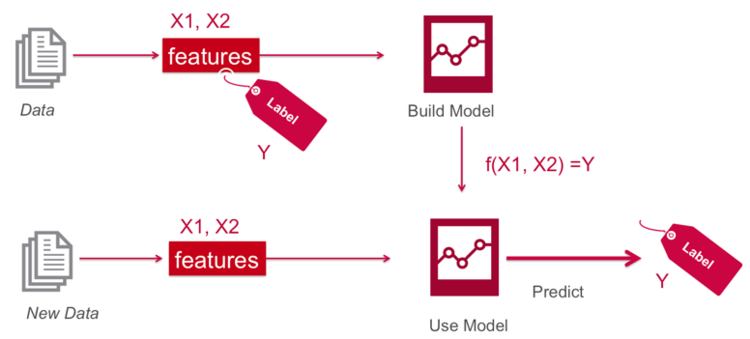
\includegraphics[width=11.9cm]{images/glossary/supervised_learning_1.png}
			%\caption{Stripe Radar for Fraud Detection}
			\label{fig:glossary_supervised_learning_1}
		\end{figure}

	\end{block}

\end{frame}


\begin{frame}

	\frametitle{Glossario}
	\framesubtitle{introduciamo alcuni termini ricorrenti nel \ml}

	\begin{block}{Modello (il caso classico dell'apprendimento supervisionato)}
		\begin{figure}[!htbp]
			\centering
			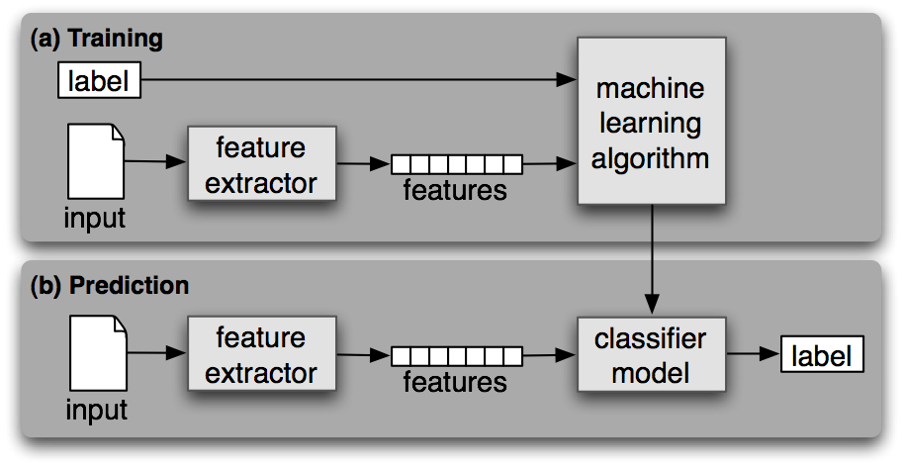
\includegraphics[width=11.2cm]{images/glossary/supervised_learning_2.png}
			\label{fig:glossary_supervised_learning_2}
			%\caption{Stripe Radar for Fraud Detection}
		\end{figure}

	\end{block}

\end{frame}


\ifthenelse{\boolean{highschool}}{}{
% https://medium.com/@dataakkadian/what-are-parametric-vs-nonparametric-models-8bfa20726f4d
\subsection[Modelli: parametrici vs non parametrici]{Modelli: parametrici vs non parametrici}

\begin{frame}

	\frametitle{Modelli: parametrici vs non parametrici}

	\begin{block}{Modelli: parametrici vs non parametrici}
		In base alle assunzioni che uno specifico modello stabilisce è possibile separare i modelli di machine learning in due categorie:
		\begin{itemize}
			\item modelli di tipo \textbf{parametrico}
			\item modelli di tipo \textbf{non parametrico}
		\end{itemize}
	\end{block}

\end{frame}


\subsubsection[Modelli Parametrici]{Modelli Parametrici}

\begin{frame}

	\frametitle{Modelli Parametrici}

	%\begin{block}{}
		\begin{itemize}
			\item riassumono i dati tramite un insieme finito di parametri $\theta$,\\
				indipendentemente dal numero di esempi di addestramento
			\item indipendentemente dalla quantità di dati forniti a un modello parametrico, questo non cambierà idea sul numero di parametri necessari per descrivere i dati
			\item quindi la complessità del modello è limitata anche se la quantità di dati è illimitata, questo li rende per certi versi \textbf{poco flessibili}
			\item i modelli parametrici asssumono una forma funzionale specifica per $f$, che dipende da un piccolo numero di $p$ \emph{parametri} ignoti:\\
				$$\theta = (\theta_1,\theta_2,\ldots,\theta_p)^\prime$$
			\item un modello parametrico può essere reso \emph{molto flessibile} aumentando il numero di parametri $p$
		\end{itemize}
	%\end{block}

\end{frame}





% TODO Valutare per caso mancasse un theta con 0 qui nel modello e nel predittore
\begin{frame}
	\frametitle{Modelli Parametrici}

	\begin{block}{Un esempio: la regressione lineare}
		\begin{itemize}
		\item esempio: Regressione lineare\\
	  			\makebox[\textwidth]{$f(X_i) = \theta_1 X_{i1}+\theta_2 X_{i2} + \ldots + \theta_p X_{ip}$}\\
			\vspace{2mm}
			\item usiamo il campione per \emph{stimare} $\theta$ o \emph{addestrare (fit/train)} il modello. Di solito per farlo ottimizziamo una misura dell'adattamento ai dati
			\item esempio: Minimi quadrati $\widehat\theta = (\mbX^\prime \mbX)^{-1} \mbX' \bfy = \mbX^{+}\bfy$\\
			(un metodo di stima \emph{globale}, dove $X^{+}$ è la matrice pseudoinversa di Moore-Penrose di $X$)
		\item Il \emph{predittore} è dato da
			$$\widehat{f}(X_0) = \widehat{\theta}_1 X_{i1} + \widehat{\theta}_2 X_{i2} + \ldots + \widehat{\theta}_p X_{ip}$$
		\end{itemize}
	\end{block}
\end{frame}


\subsubsection[Modelli Non Parametrici]{Modelli Non Parametrici}

\begin{frame}

	\frametitle{Modelli Non Parametrici}

	%\begin{block}{}
		\begin{itemize}
			\item non richiedono una ipotesi sulla forma di $f$
			\item sono utili quando si hanno molti dati e nessuna conoscenza precedente e quando non ci si vuole preoccupare troppo di scegliere le features giuste
			\item presuppongono che la distribuzione dei dati non possa essere definita in termini di un insieme finito di parametri.\\
				Ma spesso possono essere definiti assumendo un $\theta$ di dimensione infinita. Solitamente pensando a $\theta$ come ad una funzione
			\item la quantità di informazioni che $\theta$ può acquisire sui dati $D$ può aumentare al crescere della quantità di dati, questo li rende \textbf{più flessibili}
		\end{itemize}

	%\end{block}

\end{frame}


\subsubsection[Alcuni tradeoff]{Alcuni tradeoff}

\begin{frame}
	\frametitle{Alcuni tradeoff}
	\begin{itemize}
		\item Un modello parametrico può non essere abbastanza flessibile da adattarsi sufficientemente bene ai dati
		\item L'adattamento ai dati può essere migliorato usando un metodo più flessibile
		\item Ma questo non è sempre consigliabile
			\begin{enumerate}
				\item Un modello flessibile è più difficile da interpretare di un altro più semplice
					\begin{itemize}
						\item[--] i modelli lineari sono facili da interpretare, a differenza per es. di KNN
					\end{itemize}
				\item Un modello flessibile può adattarsi molto bene ai dati \emph{nel campione} ma prevedere molto male \emph{al di fuori di esso}; in altre parole può essere affetto da \emph{overfit}
					\begin{itemize}
						%\item notare che l'errore irriducibile $\Var(\varepsilon)$ non può essere ridotto
						\item[--] come possiamo sapere se l'adattamento ai dati nel campione di stima \`{e} adeguato?
					\end{itemize}
				\item Principio di parsimonia
					\begin{itemize}
						\item in generale, è sempre meglio preferire un modello con poche variabili rispetto a un predittore che ne usa molte in maniera non molto chiara e trasparente
					\end{itemize}
			\end{enumerate}
	\end{itemize}
\end{frame}


\begin{frame}

	\frametitle{Modelli: parametrici vs non parametrici}

	\begin{block}{Modelli: parametrici vs non parametrici}
		In conclusione con i modelli parametrici per effettuare delle nuove previsioni, è sufficiente conoscere i parametri del modello.
		\newlinedouble
		I metodi non parametrici sono più flessibili e per effettuare delle nuove previsioni è necessario conoscere i parametri del modello e lo stato dei dati che sono stati osservati.
	\end{block}

\end{frame}
}





\subsection[Tipi di apprendimento]{Tipi di apprendimento}
\begin{frame}

	\frametitle{Le tipologie di apprendimento}

	\begin{block}{Machine Learning, altre definizioni}
		$\Rightarrow$ computational statistics\\
		$\Rightarrow$ building computational artifacts that learn over time based on experience
	\end{block}

	\begin{block}{Le tipologie di apprendimento}

		Le tecniche di Machine Learning sono generalmente suddivise\\
		in tre grandi categorie:

		\begin{enumerate}
			\item ad apprendimento \textbf{non supervisionato} (unsupervised learning)
			\item ad apprendimento \textbf{supervisionato} (supervised learning)
			\item ad apprendimento \textbf{per rinforzo} (reinforcement learning)
		\end{enumerate}

		a seconda della natura del ``segnale'' utilizzato per l'apprendimento.
	\end{block}


\end{frame}


\begin{frame}

	\frametitle{Le tipologie di apprendimento}

	\begin{figure}[!htbp]
		\centering
		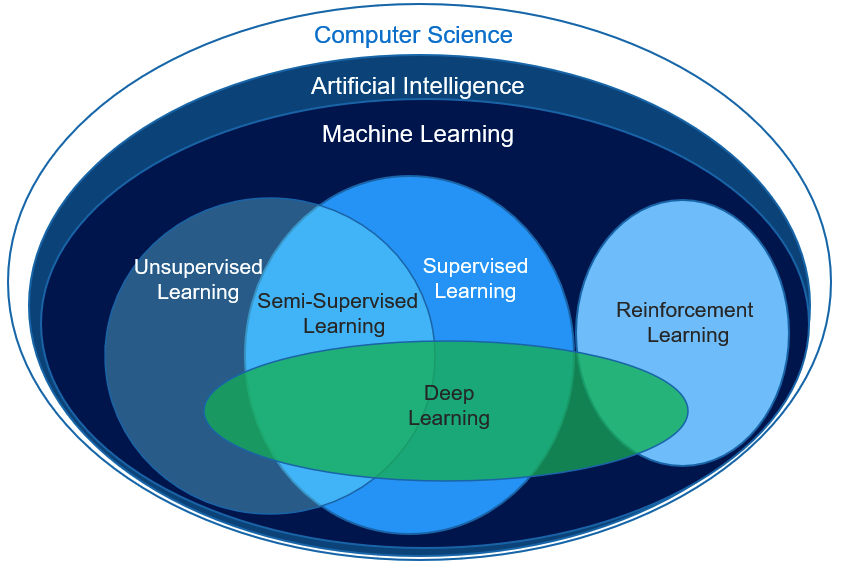
\includegraphics[width=10cm]{images/glossary/learning_types.png}
		%\caption{Stripe Radar for Fraud Detection}
	\end{figure}

\end{frame}


\subsubsection{Apprendimento non supervisionato}

\begin{frame}

	\frametitle{Apprendimento non supervisionato}

	\begin{block}{Qualche definizione}
		\begin{itemize}
			\item a partire da esempi non etichettati si cerca di derivare quali siano le caratteristiche che li accomunano/distinguono tra loro semplicemente osservando le relazioni che intercorrono tra gli esempi stessi
			\item questi algoritmi imparano semplicemente dagli esempi, senza che gli vengano fornite risposte associate (lables):\\
				è l'algoritmo stesso a stabilire autonomamente quali sono le caratteristiche distintive (i pattern) dei dati
			\item non vengono assegnate etichette all'algoritmo di apprendimento, lasciando che sia solo lui a trovare la struttura nel suo input.
			\item in breve ricavare una \textbf{descrizione compatta}
		\end{itemize}

	\end{block}


\end{frame}


\begin{frame}
	\frametitle{Apprendimento non supervisionato}
	\begin{block}{Osservazioni}
		\begin{itemize}
			\item può essere applicato come obiettivo in sè (osservare i dati sotto una diversa prospettiva, scoprendone nuovi significati; segmentare il mercato) o un mezzo per raggiungere un altro fine (creando nuovi input per gli algoritmi di machine learning supervisionati)
			\item si può fare un parallelo fra questi algoritmi e il modo in cui gli esseri umani cercano di comprendere che determinati oggetti o eventi appartengono alla stessa classe (effettuano associazioni sulla base del grado di somiglianza fra due oggetti)
			\item alcuni sistemi di raccomandazione presenti sul web vanno a ricercare possibili suggerimenti fra i dati relativi a ciò che avete acquistato in passato; le raccomandazioni sono basate sulla stima del gruppo di clienti a cui assomigliate di più, inferendo quindi le vostre probabili preferenze in base a tale gruppo
		\end{itemize}

	\end{block}

\end{frame}


\begin{frame}

	\frametitle{Apprendimento non supervisionato}

	\begin{block}{Un esempio di apprendimento non supervisionato: il clustering}
	
		
		\begin{columns}
			\column{0.425\linewidth}
			\begin{figure}[!htbp]
				\centering
				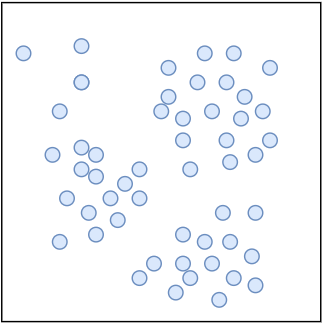
\includegraphics[width=1.0\linewidth]{images/glossary/unsupervised_learning_1_1.png}
				%\caption{}
			\end{figure}
			
			\column{0.05\linewidth}
			\begin{Huge}
				$$\pmb{\Rightarrow}$$
			\end{Huge}
			
			\pause

			\column{0.425\linewidth}
			\begin{figure}[!htbp]
				\centering
				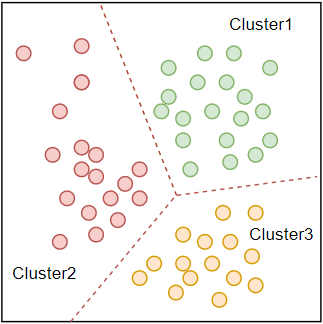
\includegraphics[width=1.0\linewidth]{images/glossary/unsupervised_learning_1_2.png}
				%\caption{}
			\end{figure}	
		\end{columns}

	\end{block}

\end{frame}


\begin{frame}

	\frametitle{Apprendimento non supervisionato}

	\begin{block}{Un esempio di apprendimento non supervisionato: il clustering}
	
		\begin{columns}
			\column{0.425\linewidth}
			\begin{figure}[!htbp]
				\centering
				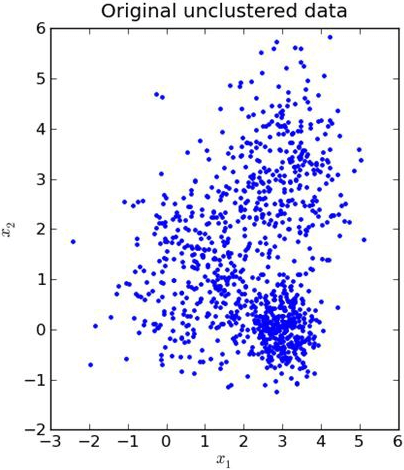
\includegraphics[width=1.0\linewidth]{images/glossary/unsupervised_learning_2_1.png}
				%\caption{Stripe Radar for Fraud Detection}
			\end{figure}
			
			\column{0.05\linewidth}
			\begin{Huge}
				$$\pmb{\Rightarrow}$$
			\end{Huge}
			
			\pause
			
			\column{0.425\linewidth}
			\begin{figure}[!htbp]
				\centering
				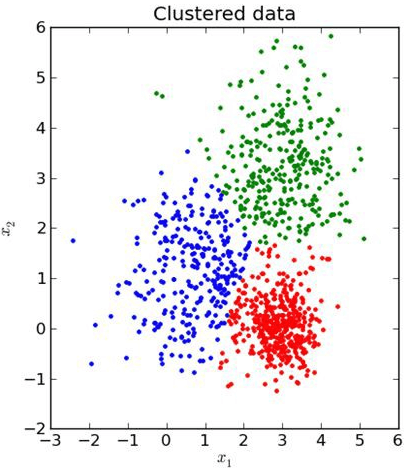
\includegraphics[width=1.0\linewidth]{images/glossary/unsupervised_learning_2_2.png}
				%\caption{Stripe Radar for Fraud Detection}
			\end{figure}	
		\end{columns}

	\end{block}

\end{frame}


\begin{frame}

	\frametitle{Apprendimento non supervisionato}

	\begin{block}{Un esempio di apprendimento non supervisionato con il \textbf{Mean Shift}}
		\begin{figure}[!htbp]
			\centering
			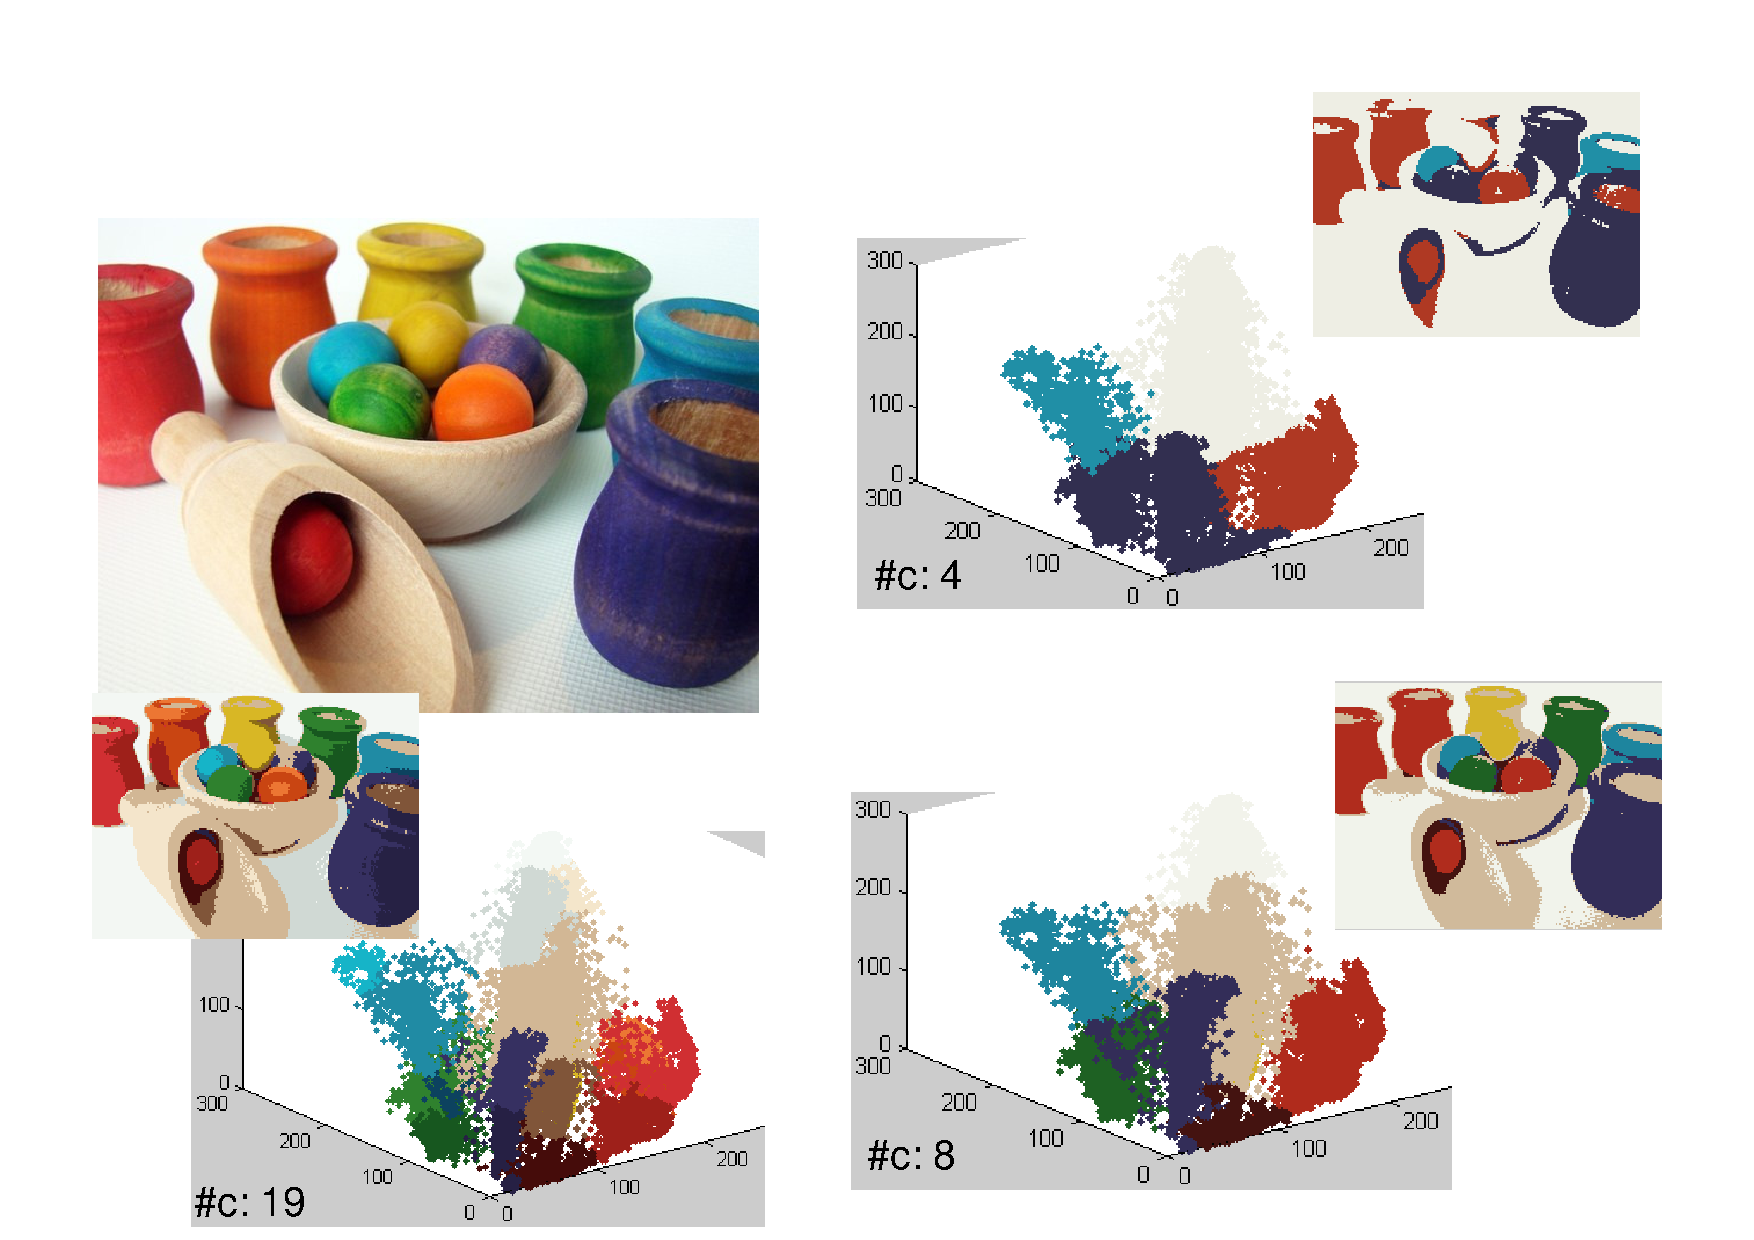
\includegraphics[width=8.5cm]{images/unsupervised/non_parametric/meanshift_pots.pdf}
			%\caption{Stripe Radar for Fraud Detection}
		\end{figure}

	\end{block}

\end{frame}



\subsubsection{Apprendimento supervisionato}
\begin{frame}

	\frametitle{Apprendimento supervisionato}

	\begin{block}{Qualche definizione}
		\begin{itemize}
			\item un algoritmo che impara da dati di esempio associati a risposte già pronte.\\
				Lo scopo di questo apprendimento è fare in modo che, quando all'algoritmo vengono sottoposti nuovi esempi, l'algoritmo stesso sia in grado di prevedere le risposte corrette
			\item prendere un dataset etichettato (labeled), indurre una regola generale per riuscire ad etichettare un nuovo dataset sprovvisto di etichette (unlabeled)
			\item vengono presentati degli input di esempio con associati  degli output desiderati, forniti da un ``insegnante'', e l'obiettivo è quello di apprendere una regola generale che mappa gli input sugli output
			\item in breve \textbf{functional approximation}
		\end{itemize}
	\end{block}

\end{frame}


\begin{frame}

	\frametitle{Apprendimento supervisionato}

	%\begin{block}{}

		Se vi viene data la seguente tabella:
		\begin{table}[]
			\begin{tabular}{ccccccccccc}
				\multicolumn{1}{c|}{input} 		& 1 & 2 & 3 & 4 & 5 & 6 & 7 & & 10 &  \\ \hline
				\multicolumn{1}{l|}{output}     & \undermat{labeled}{1 & 4 & 9 & 16 & 25 & 36 & 49 &} \undermat{unlabeled}{& ? &}  \\
			\end{tabular}
		\end{table}
		\vspace{5mm}

		\pause
		Molto probabilmente inferirete che la/il regola/modello è la/il seguente:
		$$output \leftarrow input^2 $$
		% Ma per affermare questo si fa un salto di fede (leap of faith)
		\pause
		Tuttavia esistono una miriade di altre regole/modelli che risultano essere comunque coerenti con il mapping mostrato (labeled):
		\begin{itemize}
			\item $output \leftarrow input^2$ eccetto per 10
			\item $output \leftarrow input^2$ per input tra 1 e 7; $output \leftarrow input$ altrimenti
			\item etc
		\end{itemize}


	%\end{block}



\end{frame}

\begin{frame}

	\frametitle{Apprendimento supervisionato}

	\begin{block}{Il problema della generalizzazione}
		Per utilizzare l'apprendimento supervisionato è necessario fare una assunzione fondamentale, ovvero che, attraverso i dati, sia possibile fare delle \textbf{generalizzazioni}.\\
	\end{block}

	\pause

	\begin{block}{Bias e inductive bias}
		Tutto il \ml e più nello specifico l'apprendimento supervisionato è basato sull'\textbf{induzione}.\\
		\textbf{Induzione}: passare da esempi ad una regola più generale,\\
		\hspace{31mm} dallo specifico al generale.
		\newlinedouble
		L'\textbf{inductive bias} (noto anche come \textbf{learning bias}) di un algoritmo di apprendimento è l'insieme delle assunzioni che il \textbf{learner} utilizza per\\ predire \textit{output} a partire da dati di \textit{input} che non ha ancora incontrato.
	\end{block}



\end{frame}

%\subsection[Glossario]{Glossario}



\begin{frame}

	\frametitle{Apprendimento supervisionato}

	\begin{block}{Deduction}
		L'induzione si contrappone alla \textbf{deduzione}, che consiste nel portare, tramite un ragionamento,
		da una regola generale ad uno più specifico.
		\newlinedouble
		Ad esempio: $A \implies B$, se $A$ è vero allora posso affermare che $B$ è vero.

	\end{block}


\end{frame}



\begin{frame}

	\frametitle{Apprendimento supervisionato}

	\begin{block}{Regressione vs. classificazione}
		L'apprendimento supervisionato può essere ulteriormente\\
		suddiviso in \textbf{due tipologie}:

		\begin{itemize}
			\item \textbf{modelli di regressione} che prevedono valori continui.\\
				\vspace{2mm}
				Ad esempio, i modelli di regressione fanno previsioni che rispondono a domande come le seguenti:
				\begin{itemize}
					\item[--] qual è il valore di una casa in California?
					\item[--] qual è la probabilità che un utente faccia clic su questo annuncio?
				\end{itemize}
				\vspace{2mm}
			\item \textbf{modelli di classificazione} che prevedono valori discreti.\\
				\vspace{2mm}
				Ad esempio, i modelli di classificazione fanno previsioni che rispondono a domande come le seguenti:
				\begin{itemize}
					\item[--] un determinato messaggio di posta elettronica è spam o non è spam?
					\item[--] è l'immagine di un cane, un gatto o un criceto?
				\end{itemize}
		\end{itemize}
	\end{block}


\end{frame}


\begin{frame}

	\frametitle{Apprendimento supervisionato}

	\begin{block}{Regressione vs. classificazione ($T_{C^{\circ}} = (T_{F^{\circ}} - 32) \times \frac{5}{9}$)}
		\begin{figure}[!htbp]
			\centering
			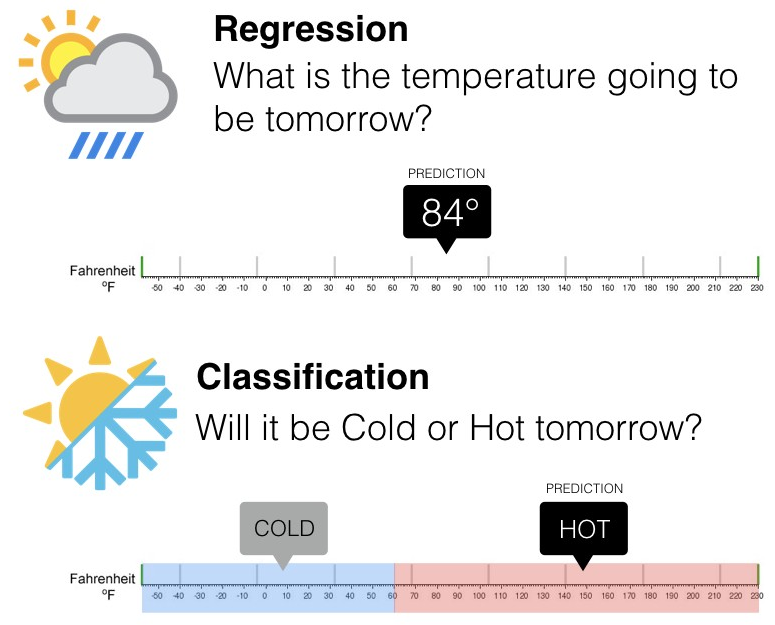
\includegraphics[width=7cm]{images/glossary/regression_vs_classification_2.png}
			%\caption{Stripe Radar for Fraud Detection}
		\end{figure}

	\end{block}

\end{frame}


\begin{frame}

	\frametitle{Apprendimento supervisionato}

	% Es twitter followers --> salary (for regression)
	\begin{block}{Regressione vs. classificazione}
		\begin{figure}[!htbp]
			\centering
			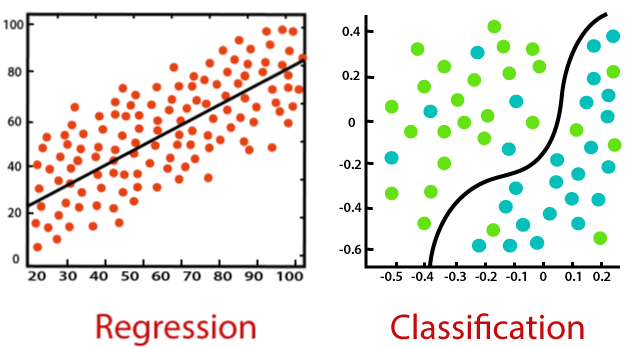
\includegraphics[width=10cm]{images/glossary/regression_vs_classification_1.png}
			%\caption{Stripe Radar for Fraud Detection}
		\end{figure}

	\end{block}

\end{frame}



\begin{frame}

	\frametitle{Glossario}
	\framesubtitle{introduciamo alcuni termini ricorrenti nel \ml}

	\begin{block}{Modello (il caso classico dell'apprendimento supervisionato)}
		\begin{figure}[!htbp]
			\centering
			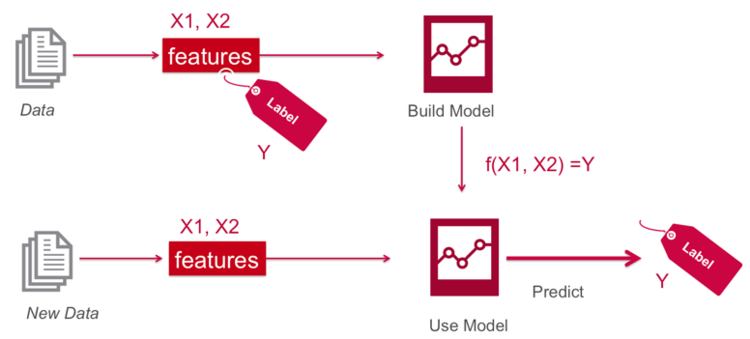
\includegraphics[width=11.9cm]{images/glossary/supervised_learning_1.png}
			%\caption{Stripe Radar for Fraud Detection}
			\label{fig:glossary_supervised_learning_1}
		\end{figure}

	\end{block}

\end{frame}


\begin{frame}

	\frametitle{Glossario}
	\framesubtitle{introduciamo alcuni termini ricorrenti nel \ml}

	\begin{block}{Modello (il caso classico dell'apprendimento supervisionato)}
		\begin{figure}[!htbp]
			\centering
			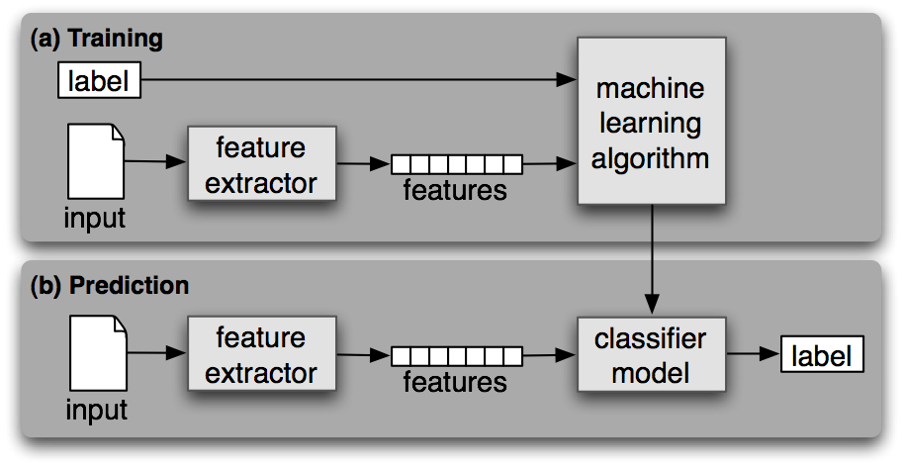
\includegraphics[width=11.2cm]{images/glossary/supervised_learning_2.png}
			\label{fig:glossary_supervised_learning_2}
			%\caption{Stripe Radar for Fraud Detection}
		\end{figure}

	\end{block}

\end{frame}


\begin{frame}

	\frametitle{Apprendimento: supervisionato vs non supervisionato}

	\begin{block}{}
		\begin{figure}[!htbp]
			\centering
			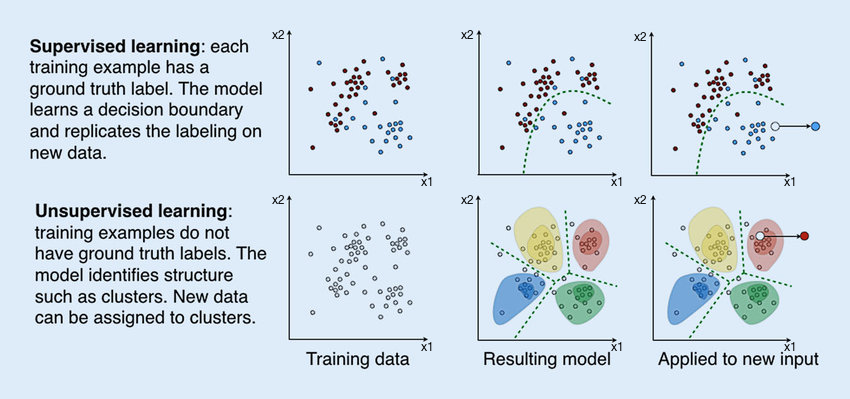
\includegraphics[width=12cm]{images/glossary/supervised_vs_unsupervised_1.png}
			%\caption{Stripe Radar for Fraud Detection}
		\end{figure}

	\end{block}

\end{frame}


\begin{frame}

	\frametitle{Apprendimento: supervisionato vs non supervisionato}

	\begin{block}{}
		\begin{figure}[!htbp]
			\centering
			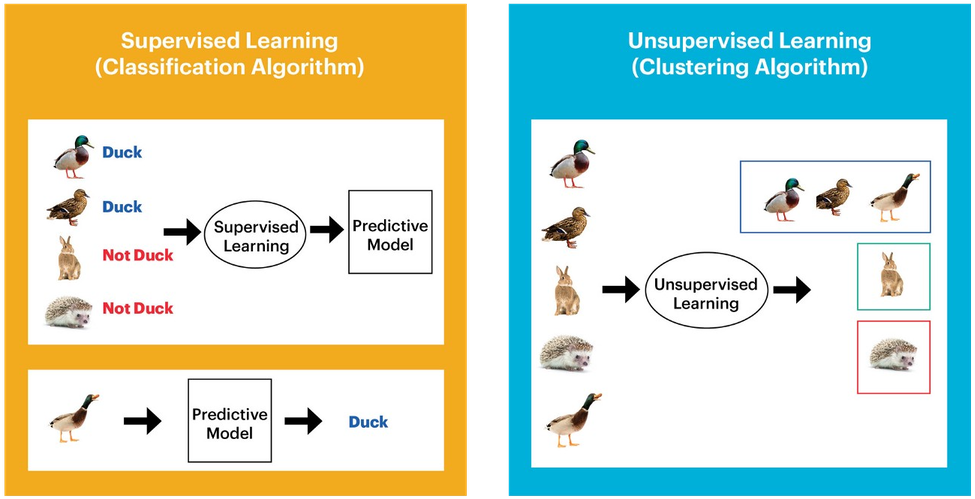
\includegraphics[width=12cm]{images/glossary/supervised_vs_unsupervised_2.png}
			%\caption{Stripe Radar for Fraud Detection}
		\end{figure}

	\end{block}

\end{frame}


\begin{frame}

	\frametitle{Apprendimento: supervisionato vs non supervisionato}

	\begin{block}{}
		\begin{figure}[!htbp]
			\centering
			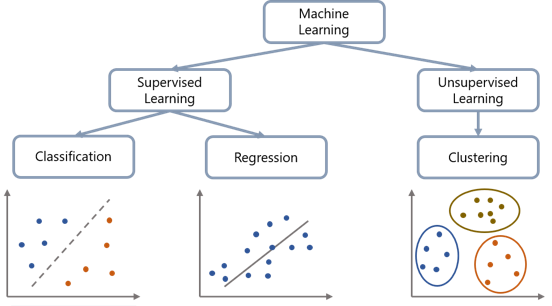
\includegraphics[width=12cm]{images/glossary/supervised_vs_unsupervised_3.png}
			%\caption{Stripe Radar for Fraud Detection}
		\end{figure}

	\end{block}

\end{frame}



\ifthenelse{\boolean{highschool}}{}{
	\subsubsection{Apprendimento per rinforzo}
	
	\begin{frame}
	
		\frametitle{Apprendimento per rinforzo}
	
		\begin{block}{Qualche definizione}
			\begin{itemize}
				\item si presentano all'algoritmo degli esempi privi di risposta associata, come nell'apprendimento non supervisionato; l'algoritmo può però proporre una soluzione agli esempi e \textbf{ricevere un feedback positivo o negativo} dal quale apprendere. L'apprendimento per rinforzo viene utilizzato con le applicazioni nelle quali l'algoritmo deve prendere delle decisioni da cui discendono delle conseguenze (pertanto il risultato dell'apprendimento è di tipo prescrittivo, cioè indica che cosa si dovrebbe fare, e non soltanto descrittivo, come invece accade nell'apprendimento non supervisionato)
				\item il modello interagisce con un ambiente dinamico nel quale cerca di raggiungere un obiettivo (per esempio guidare un veicolo), avendo un insegnante che gli dice solo se ha raggiunto l'obiettivo
				\item in breve \textbf{learning from delayed reward}
			\end{itemize}
	
		\end{block}
	
	
	\end{frame}
	
	
	\begin{frame}
	
		\frametitle{Apprendimento per rinforzo}
	
		\begin{block}{Osservazioni}
			\begin{itemize}
				\item nel mondo umano, è un po' come imparare con prove ed errori: gli ultimi aiutano a imparare, perché il fatto che vi sia implicato un costo (in termini economici, ma anche di perdita di tempo, dispiacere, dolore e così via) insegna che una certa linea di condotta ha potenzialmente meno probabilità di riuscita rispetto ad altre
				\item un interessante esempio di \textbf{apprendimento per rinforzo} si verifica quando i computer imparano autonomamente a giocare a un videogioco.\\
				In questo caso, un'applicazione presenta all'algoritmo degli esempi di situazioni specifiche di gioco. L'applicazione fa conoscere all'algoritmo il risultato delle azioni che potrebbe intraprendere e l'apprendimento si verifica allorché l'algoritmo cerca di evitare ciò che scopre essere pericoloso e cerca di continuare a sopravvivere nel gioco.
			\end{itemize}
		\end{block}
	
	\end{frame}
	
	
	\begin{frame}
	
		\frametitle{Apprendimento per rinforzo}
	
		\begin{block}{Osservazioni}
	
			\begin{columns}
	
				\column{0.6\linewidth}
				\begin{itemize}
					\item Su YouTube all'indirizzo \href{https://www.youtube.com/watch?v=V1eYniJ0Rnk}{\underline{Google DeepMind's Deep Q-learning playing Atari Breakout}} potete osservare in che modo \textbf{DeepMind} ha sviluppato un programma di apprendimento per rinforzo che gioca a un videogame Atari del passato. Osservando il video, si nota che, all'inizio, il programma è piuttosto imbranato e non particolarmente abile nel gioco, ma attraverso l’apprendimento migliora a mano a mano, fino a diventare un campione
				\end{itemize}
	
				\column{0.4\linewidth}
				\begin{figure}[!htbp]
					\centering
					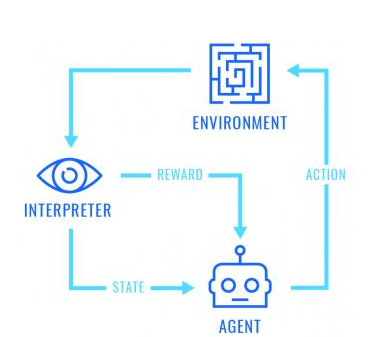
\includegraphics[width=5cm]{images/glossary/reinforcement_learning.png}
					%\caption{Stripe Radar for Fraud Detection}
				\end{figure}
	
			\end{columns}
	
		\end{block}
	
	\end{frame}


	\begin{frame}
	
		\frametitle{Le tipologie di apprendimento}
	
		\begin{block}{L'ottimizzazione}
				Tutte queste categorie di apprendimento automatico sono \textbf{interconnesse}.\\
				Infatti si potrebbe formulare ognuno di questi problemi sottoforma di un \textbf{problema di ottimizzazione}:
				\begin{figure}[!htbp]
					\centering
					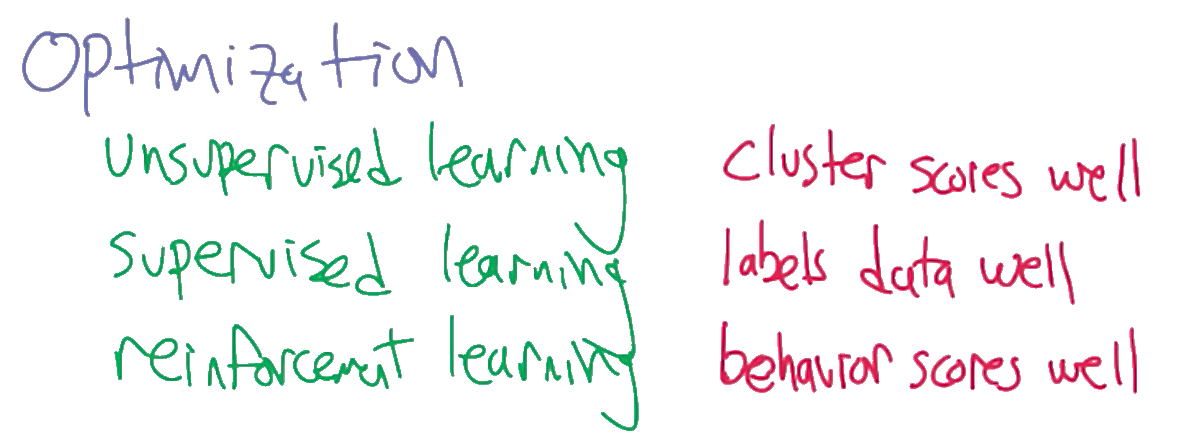
\includegraphics[width=11cm]{images/glossary/optimization.png}
					%\caption{Stripe Radar for Fraud Detection}
				\end{figure}
		\end{block}
	
	\end{frame}
}